\documentclass[10pt]{article}

\usepackage{fancyhdr}
\usepackage{extramarks}
\usepackage{amsmath}
\usepackage{amsthm}
\usepackage{amsfonts}
\usepackage{tikz}
\usepackage{ragged2e}
\usetikzlibrary{automata,positioning}
\usepackage{setspace}
\usepackage{etoolbox}
\usepackage{enumitem}
\usepackage{hyperref}
\hypersetup{colorlinks=true,allcolors=blue}
\usepackage{hypcap}
\usepackage{graphicx}    %for figure environment.
\usepackage{calc}
\usepackage{ifthen}
\usepackage{tikz}
\usepackage{longtable}
\usepackage{lipsum}
\usepackage{verbatim}
\usepackage{enumitem}
\setlist[enumerate]{itemsep=0mm}
\setlist[itemize]{itemsep=0mm}
\usepackage{pstricks-add}
\usepackage{pstricks}
\usepackage{rotating}
\usepackage[]{algorithm2e}
\usepackage{pdfpages}


\makeatletter
\pretocmd{\@sect}{\singlespacing}{}{}
\pretocmd{\@ssect}{\singlespacing}{}{}
\apptocmd{\@sect}{\singlespacing}{}{}
\apptocmd{\@ssect}{\singlespacing}{}{}
\makeatother

%
% Basic Document Settings
%
\newcommand{\ts}{\textsuperscript}

%\begin{comment}
\topmargin=-0.45in
\evensidemargin=0in
\oddsidemargin=0in
\textwidth=6.5in
\textheight=9.0in
\headsep=0.25in
%\end{comment}

\linespread{1.1}

\pagestyle{fancy}
\lhead{\hmwkAuthorName}
\chead{\textbf{\hmwkClass : \hmwkTitle}}
\rhead{\hmwkAuthorNumber}
\lfoot{\lastxmark}
\cfoot{\thepage}

\renewcommand\headrulewidth{0.4pt}
\renewcommand\footrulewidth{0.4pt}

\setlength\parindent{0pt}

%
% Create Problem Sections
%


\setcounter{secnumdepth}{0}
\newcounter{partCounter}
\newcounter{homeworkProblemCounter}
\setcounter{homeworkProblemCounter}{1}
\nobreak\extramarks{Problem \arabic{homeworkProblemCounter}}{}\nobreak{}

%
% Homework Problem Environment
%
% This environment takes an optional argument. When given, it will adjust the
% problem counter. This is useful for when the problems given for your
% assignment aren't sequential. See the last 3 problems of this template for an
% example.
%


%
% Homework Details
%   - Title
%   - Due date
%   - Class
%   - Section/Time
%   - Instructor
%   - Author
%

\newcommand{\hmwkTitle}{Assignment 3\ \ }
\newcommand{\hmwkDueDate}{Sunday, December 3\ts{rd}, 2017}
\newcommand{\hmwkClass}{CSC411}
\newcommand{\hmwkClassTime}{Section A}
\newcommand{\hmwkClassInstructor}{Steven Chuang}
\newcommand{\hmwkClassTeachingAssistant}{Natalia Mykhaylova}
\newcommand{\hmwkAuthorName}{Gokul K. Kaushik}
\newcommand{\hmwkAuthorNumber}{999878191}
\newcommand{\schoolmate}{\textsc{School-Mate }}

\newcommand\Tstrut{\rule{0pt}{2.6ex}}       % "top" strut
\newcommand\Bstrut{\rule[-0.9ex]{0pt}{0pt}} % "bottom" strut
\newcommand{\TBstrut}{\Tstrut\Bstrut} % top&bottom struts
%
% Title Page
%

\title{
    \vspace{2in}
    \textmd{\textbf{\hmwkClass:\ \hmwkTitle}}\\
    \vspace{0.1in}\small{Due\ on\ \hmwkDueDate}\\
    \vspace{3in}
    \vspace{0.1in}\large{Student Name: \textbf{\hmwkAuthorName} } \\
    \vspace{0.1in}\large{Student Number: \textbf{\hmwkAuthorNumber} } \\
}

%\author{\textbf{\hmwkAuthorName}}
%\textbf{\hmwkAuthorNumber\}
\date{}

\renewcommand{\part}[1]{\textbf{\large Part \Alph{partCounter}}\stepcounter{partCounter}\\}

%
% Various Helper Commands
%

% Useful for algorithms
\newcommand{\alg}[1]{\textsc{\bfseries \footnotesize #1}}

% For derivatives
\newcommand{\deriv}[1]{\frac{\mathrm{d}}{\mathrm{d}x} (#1)}

% For partial derivatives
\newcommand{\pderiv}[2]{\frac{\partial}{\partial #1} (#2)}

% Integral dx
\newcommand{\dx}{\mathrm{d}x}

% Alias for the Solution section header
\newcommand{\solution}{\textbf{\large Solution}}

% Probability commands: Expectation, Variance, Covariance, Bias
\newcommand{\E}{\mathrm{E}}
\newcommand{\Var}{\mathrm{Var}}
\newcommand{\Cov}{\mathrm{Cov}}
\newcommand{\Bias}{\mathrm{Bias}}
\renewcommand*\contentsname{Table of Contents}

\begin{document}
\maketitle
\pagebreak

\begin{center} \tableofcontents \end{center}
\pagebreak

\clearpage
\setcounter{page}{1}

\section{1 - 20 Newsgroup Predictions}
\section{2 - Training SVM with SGD}
\subsection{2.1 - SGD with Momentum}

Plotting $w_t$ for each time step $t$ by applying the iterative stochastic gradient-descent on $ f(w) = 0.01w^2$, we get the following graph (for $\beta = 0.1$ and $\beta = 0.9$ for upto 200 time-steps):

\begin{center}
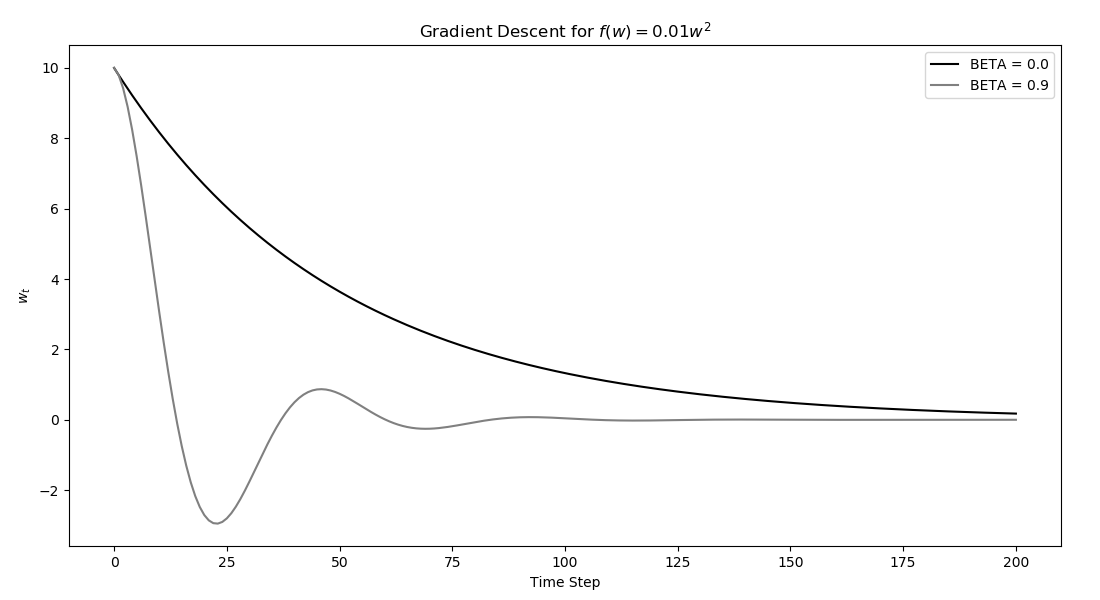
\includegraphics[scale=0.5]{2_1.png}
\end{center}



\subsection{2.2 -Training SVM}
\subsection{2.3 - Apply 4-vs-9 Digits on MNIST}
\subsubsection{2.3.1 - Training Loss}
\subsubsection{2.3.2 - Test Loss}
\subsubsection{2.3.3 - Classification Accuracy on the Training Set}
\subsubsection{2.3.4 - Classification Accruacy on the Test Set}
\subsubsection{2.3.5 - Plot \textbf{$w$} as a 28 $\times $ 28 image }


\section{3 - Kernels}
\subsection{3.1 - Positive Semi definite and Quadratic Form}

Prove that a symmetric matrix $K \in \mathbb{R}^{d \times d} $ is a positive semi definite iff for all vectors $x$ we have $\textbf{x}^{T}K\textbf{x} \geq 0$.
\\ \\
Proof: 

\[
K\textbf{x} = \lambda \textbf{x}
\]

where $\lambda$ is the eigenvalue and $\textbf{x}$ is the eigenvector. 
\\ \\
Suppose $\textbf{x}$ is an eigenvector of $K$ and replacing $K\textbf{v}$ with $\lambda \textbf{v}$ (from the definition of an eigenvector and eigenvalue above):
\[
\textbf{x}^{T}K\textbf{x} = \textbf{x}^{T} \textbf{x} \lambda
\]

\[
\textbf{x}^{T}K\textbf{x} = |\textbf{x}|^{2} \lambda
\]

Therefore, as $|\textbf{x}|^{2} \geq 0$, for the equation $\textbf{x}^{T}K\textbf{x} \geq 0$, the eigenvalue must be: $\lambda \geq 0$. Since it is a semi-definite matrix, where the eigenvalues $\geq 0$, this holds true.  


\subsection{3.2 - Kernel Properties}
\subsubsection{3.2.1 - Prove Property $k(\textbf{x},\textbf{y}) = \alpha $ is a kernel for $\alpha > 0$}

\[
\phi(\textbf{x}) = \sqrt{\alpha}
\]

\[
k(\textbf{x},\textbf{y}) = \langle \phi(\textbf{x}), \phi(\textbf{y}) \rangle
\]

\[
k(\textbf{x},\textbf{y}) = \sqrt{\alpha} \sqrt{\alpha}
\]

\[
k(\textbf{x},\textbf{y}) = \alpha
\]

\subsubsection{3.2.2 - Prove Property $k(\textbf{x},\textbf{y}) = f(\textbf{x}) \cdot f(\textbf{y}) $ is a kernel for $ f: \mathbb{R}^{d} \rightarrow \mathbb{R}$}

\[
\phi(\textbf{x}) = f(\textbf{x})
\]

\[
k(\textbf{x},\textbf{y}) = \langle \phi(\textbf{x}), \phi(\textbf{y}) \rangle
\]

\[
k(\textbf{x},\textbf{y}) = f(\textbf{x}) \cdot f(\textbf{y})
\]


\subsubsection{3.2.3 - Prove Property If $k_1(\textbf{x},\textbf{y})$ and $k_2(\textbf{x},\textbf{y})$ are kernels then $k(\textbf{x},\textbf{y}) = a \cdot k_1((\textbf{x},\textbf{y}) + b \cdot k_2((\textbf{x},\textbf{y})$ for $a,b > 0$ is a kernel}

Let $\textbf{K}_1$ and $\textbf{K}_2$ be gram matrices
\\ \\
Therefore: 

\[
\textbf{x}^{T} \textbf{K}_1 \textbf{x} \geq 0
\]

and 

\[
\textbf{x}^{T} \textbf{K}_2 \textbf{x} \geq 0
\]
 
Let: 

\[
\textbf{K}_{3}(\textbf{x},\textbf{y}) = a \textbf{K}_{1}(\textbf{x},\textbf{y}) + b  \textbf{K}_{2}(\textbf{x},\textbf{y})
\]

\[
\textbf{K}_{3} = a \textbf{K}_{1} + b  \textbf{K}_{2}
\]

\[
\textbf{x}^{T} \textbf{K}_3 \textbf{x} = \textbf{x}^{T} ( a \textbf{K}_{1} + b  \textbf{K}_{2}) \textbf{x}
\]

\[
\textbf{x}^{T} \textbf{K}_3 \textbf{x} = a \textbf{x}^{T} \textbf{K}_1 \textbf{x} + b \textbf{x}^{T} \textbf{K}_2 \textbf{x}
\]

and using 3.2.1's proof, $\textbf{K}_{3}(\textbf{x},\textbf{y})$ is a kernel, we get: 

\[
a \textbf{x}^{T} \textbf{K}_1 \textbf{x} + b \textbf{x}^{T} \textbf{K}_2 \textbf{x} \geq 0 \text{ for } a,b > 0
\]


\subsubsection{3.2.3 - Prove Property If $k_1(\textbf{x},\textbf{y})$ is a kernel then $k(\textbf{x},\textbf{y}) = $ is a kernel}



\pagebreak


\end{document}

$





